\documentclass[../main/main.tex]{subfiles}

\newdate{date}{29}{11}{2019}


\begin{document}



\chapter{Non ideal fluids: Mean field theory, Van der Walls, Virial expansion and Cluster expansion}

\marginpar{ \textbf{Lecture 14.} \\  \displaydate{date}. \\ Compiled:  \today.}

\section{Mean field theory for fluids}

Ideal gases are exceedingly idealised systems and are not suited to describe the behaviour of real systems: they always obey the same state equation and never undergo phase transitions (for example they never condense). We must therefore step a little further: using the "philosophy" of mean field theories we can make the description of fluids a little bit more realistic. As we will see this will also lead to the derivation of the Van der Waals equation, which better describes the behaviour of real fluids (even if, as we will shortly see, it still has some problems).

In general, in a real gas all the atoms or molecules interact through a certain potential \(\Phi(\{\va{r}_i\})\) that will depend on the positions of all the particles. For a fluid system of  \( N \) particles  with position vectors \( \{ \va{r}_i \}_{i=1,\dots,N}   \), the configurational contribution to the (grancanonical) partition function will therefore be:

\begin{equation}
  Q_N (T) = \int_{V}^{} \prod_{i=1}^{N}  \dd[]{\va{r}_i}  e^ {-\beta  \qty( \Phi(\{\va{r}_i\}) + \sum_{i=1}^{N} \psi _{ext}  (\va{r}_i) ) }
\end{equation}
where \( \psi _{ext} \) is a one body external potential, but we do not consider it because is not the aim of our problem. In general,
\begin{equation*}
  \Phi (\{ \va{r}_i \}  ) = \sum_{i\neq j}^{}  U_2 (\va{r}_i,\va{r}_j) + \sum_{i\neq j\neq \mu }^{} U_3 (\va{r}_i, \va{r}_j, \va{r}_ \mu ) + \dots
\end{equation*}
(where \(U_{n} \) can be a generic \(n\)-body interaction potential). For simplicity, we do not consider \( U_3 \), that is the three body interaction. Let us suppose
\begin{equation*}
   U_2 (\va{r}_i,\va{r}_j) \rightarrow U_2 ( \abs{\va{r}_i - \va{r}_j} )
\end{equation*}
Therefore,
\begin{equation*}
  Q_N (T) = \int_{V}^{} \prod_{i=1}^{N}  \dd[]{\va{r}_i}  e^ {-\beta \sum_{i\neq j }^{}  U_2 ( \abs{\va{r}_i - \va{r}_j} ) }
\end{equation*}
Now, we replace all this story with just a field, it is a sort of average of the interactions. Doing the mean field assumption for \( U_2 \), we obtain
\begin{equation*}
  \sum_{i,j > 1 }^{}  U_2 ( \abs{\va{r}_i - \va{r}_j} ) \rightarrow \sum_{i}^{} \Phi _{MF} (\va{r}_i)
\end{equation*}

Generally \(\psi _{ext}\) does not pose great problems while it is \(\Phi\) that makes \( Q_{N}\) impossible to compute exactly, forcing us to resort to approximations. In the framework of mean field theories, we substitute the interaction potential \(\Phi\) with an effective single-particle potential  that acts on every particle in the same way. Hence,  the \textit{mean field approximation}  consists in substituting the multi-body interaction potential \(   \Phi (\{ \va{r}_i \}  ) \) with an effective one body potential \( \Phi (\va{r}) \) withing which all the particles move:
\begin{empheq}[box=\myyellowbox]{equation}
\Phi (\{ \va{r}_i \})   =\sum_{i}^{} \Phi _{MF} (\va{r}_i)
\end{empheq}
As said, for simplicity consider \( \psi _{ext} = 0 \), hence mean field theories allow us to compute \(Q_N\) as
\begin{equation}
  Q_N^{MF} (T) \simeq \qty[  \int_{V}^{}  \dd[D]{\va{r}}  e^ {-\beta \Phi _{MF} (\va{r})  } ]^N
\end{equation}

\begin{remark}
The integral depends on the form of \( \Phi _{MF} (\va{r})  \). Of course, every particular mean field theory will provide a different form of \( \Phi _{MF} (\va{r})  \) which will lead to different results.
\end{remark}

If one assumes \emph{spatial isotropy},
what it is important is not anymore the vector but only the distance; hence, it is important just the integral over the modulus:
\begin{equation*}
    \Phi _{MF} (\va{r}) = \Phi _{MF} (\abs{\va{r}} ) = \Phi _{MF} (r)
\end{equation*}

\section{Van der Waals equation}
The Van der Waals equation can be obtained considering the atoms of a gas as hard spheres. In this case, in fact, the mean field has the form:
\begin{equation}
\Phi _{MF} (r) =
  \begin{cases}
   \infty & r < r_0 \quad  \text{repulsion}\\
   u < 0 & r> r_0  \quad \text{attraction}
  \end{cases}
\end{equation}
as plotted in Figure \ref{fig:14_1}.
\begin{figure}[h!]
\centering
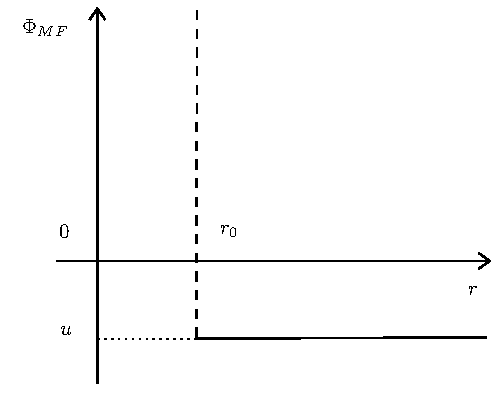
\includegraphics[width=0.6\textwidth]{../lessons/14_image/1.pdf}
\caption{\label{fig:14_1} Plot of the potential \( \Phi _{MF} (r) \).}
\end{figure}


\noindent The partition function becomes
\begin{equation*}
  Q_N^{MF} (T) = \qty[ V_{ex}e^{- \infty } + (V-V_{ex})e^{-\beta u} ]^N
\end{equation*}
where \( V_{ex} \simeq r_0^3 \) is the volume not accessible by the particle. Finally, the result is
\begin{equation}
  Q_N^{MF} (T) = \qty[ (V-V_{ex})e^{-\beta u} ]^N
\end{equation}
The free energy is \( F_N = -k_B T \ln Q_N \), hence
\begin{empheq}[box=\myyellowbox]{equation}
  F_N^{MF} (T) = - N k_B T \qty[ \ln{(V-V_{ex})} - \beta u ]
\end{empheq}
Let us calculate the pressure
\begin{equation}
  P_N^{MF} = - \eval{\pdv{F_N^{MF}}{V} }_T = \frac{N k_B T}{V-V_{ex}} - N \qty(\pdv{u}{V} )_T
  \label{eq:14_1}
\end{equation}
\begin{remark}
In general, the deep \( u \)  can go up and down depending on the \emph{V}: \( u = u (V) \). This is because \( u \) is the attractive well of the mean field potential and, for \( r \ge r_0 \) must be proportional to the fluid density
\begin{equation*}
  u \sim -N/V
\end{equation*}
where the minus sign means attraction. On the other hand, also \( V_{ex} \), the volume not accessible, must be proportional to \( N \).
\end{remark}
Hence, we have
\begin{equation*}
  u = - a \frac{N}{V}, \qquad V_{ex} = b N
\end{equation*}
where \( b \) is the volume of a single particle.
Inserting the last term in \eqref{eq:14_1}, we obtain the \emph{Van der Walls equation of state}:
\begin{empheq}[box=\myyellowbox]{equation}
  P_N^{MF} (V,T) = \frac{N k_B T}{V-bN} - a \qty(\frac{N}{V})^2
  \label{eq:14_2}
\end{empheq}



\subsection{Critical point of Van der Waals equation of state}
Let us define the specific volume as
\begin{equation*}
  v \equiv \frac{1}{\rho } = \frac{V}{N}
\end{equation*}
Hence, the equation of state becomes
\begin{equation}
P = \frac{K_B T}{v - b} - \frac{a}{v^2}
\end{equation}

The behaviour of the Van der Waals isotherms is shown in Figure \ref{fig:14_2_1}. As we can see this changes with the temperature and resembles that of real isotherms; however, Van der Waals isotherms are always analytic and have a non physical behaviour in certain regions of \( (v,P)\) plane, called spinodal curves, if \( T < T_c\): for some values of \(v\) we have \( \partial P / \partial v >0\) which is physically impossible. This is a consequence of the roughness of the approximation we have made, since it can be shown that it doesn't ensure that the equilibrium state of the system globally minimizes the Gibbs free energy. As we will shortly see, however, this problem can be solved "by hand" with Maxwell's equal area rule, or Maxwell's Construction. Overall, we have this effect because it is a mean field, so the curve in Figure \ref{fig:14_2_1} it is replaced by the curve in Figure \ref{fig:14_2_2}.
Moreover, for \( T < T_c \) the equation \( P(v) = const \) has 3 distinct solutions. For \( T > T_c \) only one solution \( \in \R \).


\begin{figure}[h!]
\begin{minipage}[c]{0.5\linewidth}
\subfloat[][ Van der Waals isotherms are represented in red in \( (v,P) \) diagram for different values of \(T\). ]{ 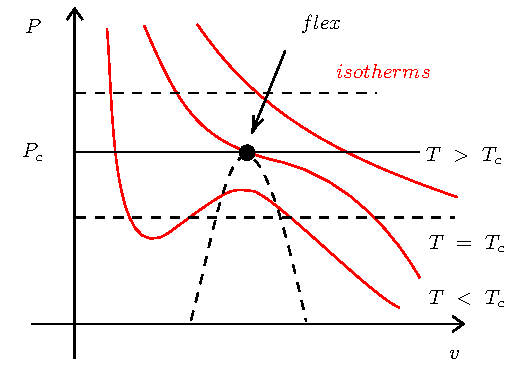
\includegraphics[width=0.9\textwidth]{../lessons/14_image/2.pdf}  \label{fig:14_2_1} }
\end{minipage}
\begin{minipage}[]{0.5\linewidth}
\centering
\subfloat[][Real isotherm in \( (v,P)\) diagram for \(T<T_c\). ]{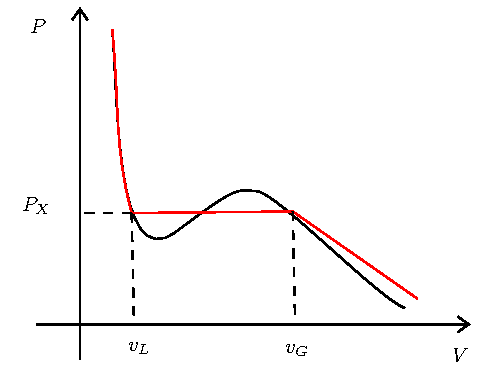
\includegraphics[width=0.9\textwidth]{../lessons/14_image/3.pdf}  \label{fig:14_2_2} }
\end{minipage}
\caption{\label{fig:} }
\end{figure}

Let us now see how to determine the critical point of a system obeying Van der Waals equation.

\begin{itemize}
\item First of all, from the representation of the isotherms we can see that the critical point is a flex for the critical isotherm (i.e. the one with \(T=T_c\)); in other words, we can determine the critical point from the equations:
\begin{equation*}
  \pdv{P}{v} = 0, \qquad \pdv[2]{P}{v} = 0
\end{equation*}
 The second in particular means that there is a flex point. Let us pay attention to it, indeed it is a standard way to find critical points.
We obtain
\begin{equation*}
  v_c = 3 b, \quad  P_c = \frac{a}{27 b^2}, \quad k_B T_c = \frac{8a}{27b}
\end{equation*}


\item Another way to find the critical point consists in noticing that at \( T=T_c \), the 3 solutions coincide. In fact, we can note that the equation \(P (v)= P = const \) is cubic in \(v\). Let us rewrite the Van der Waals equation
\begin{equation*}
  P = \frac{v^2 k_B T - a (v-b)}{v^2 (v-b)}
\end{equation*}
as
\begin{equation}
  v^3 - \qty(b + \frac{k_B T}{P})v^2 + \frac{a}{P} v - \frac{a b }{P} = 0
  \label{eq:14_3}
\end{equation}
For \(T>T_c\) this equation has one real solution and two imaginary ones, and for \(T<T_c\)  three distinct real solutions; when \(T=T_c\) the three solutions of the equation coincide. This means that at the critical point \( T=T_c \) this last equation Eq.\eqref{eq:14_3}  must be written in the form:
\begin{equation*}
  (v-v_c)^3 = 0 \quad \Rightarrow v^3 - 3 v^2 v_c + 3 v v_c^2 - v_c^3 = 0
\end{equation*}
Equating the coefficients with Eq.\eqref{eq:14_3} we get:
\begin{equation*}
  v_c^3 = \frac{a b}{P_c}, \quad 3 v_c^2 = \frac{a}{P_c}, \quad 3 v_c = b + \frac{k_B T_c}{P_c}
\end{equation*}
from which we have again:
\begin{equation}
  v_c = 3 b, \quad P_c = \frac{a}{27 b^2}, \quad k_B T_c = \frac{8 a }{27 b }
  \label{eq:14_4}
\end{equation}
We have found a very interesting result: in fact, if we can measure \(a\) and \(b\) at high temperatures then we are able to determine the critical point of the system.

This model has also an interesting property, since it predicts that:
\begin{equation*}
    \frac{P_c v_c}{k_B T_c} = \frac{3}{8}  \approx 0.375
\end{equation*}
which is a universal number, independent of \(a\) and \(b\) and so of the particular fluid considered. Experimentally this ratio is approximately 0.29 for Argon, 0.23 for water and 0.31 for  \( \text{He}^4 \).
Therefore, even if it is very rough, this model leads to reasonable conclusions.

\end{itemize}



\subsection{Law of corresponding states}
The universal value of the ratio \( \frac{P_c v_c}{k_B T_c} \) suggests a deeper correspondence between different fluid systems.
We can also rewrite Van der Waals equation \eqref{eq:14_2} in a dimensionless form, rescaling the thermodynamic quantities of the system. In particular, defining:
\begin{equation}
  \pi \equiv \frac{P}{P_c}= P\frac{27b^2}{a}, \quad \nu  \equiv \frac{v}{v_c} = \frac{v}{3b}, \quad \tau \equiv \frac{T}{T_c} = k_B T\frac{27b}{8a}
\end{equation}
Van der Waals equation becomes:
\begin{empheq}[box=\myyellowbox]{equation}
  \qty(\pi + \frac{3}{\nu ^2}) \qty(3 \nu -1) = 8 \tau
\end{empheq}
We have found another very interesting result: when rescaled by their critical thermodynamic properties (by \( P_c, v_c \) and \( T_c \)), all fluids obey the same state equation. This is the law of corresponding states: this is a form of universality. The law of corresponding states applies everywhere on the phase diagram. It can even be shown that this law is a consequence of dimensional analysis, and is more general than what might seem: experimentally the law of corresponding states is well satisfied also by fluids which do not obey Van der Waals equation.



\subsection{Region of coexistence and Maxwell's equal area rule}
In real fluids, for \( T < T_c \) \( (\tau < 1) \), there is a first order liquid-gas transition with coexistence between vapor and liquid phase and non analiticity of the thermodynamic potential. In particular, a real isotherm for \( T < T_c \) is the one in Figure \ref{fig:14_2_2}. How this is described by the mean-field (i.e. Van der Walls) theory?
The Van der Walls isotherm for \(T<T_c\) is given by the graphic in Figure \ref{fig:14_3}.
The liquid phase goes into a phase region that is not thermodinamycally stable.
How can we remove the non physical regions of the Van der Walls equation of state and describe coexistence? The solution is the Maxwell (or equal area) construction!

\begin{figure}[h!]
\centering
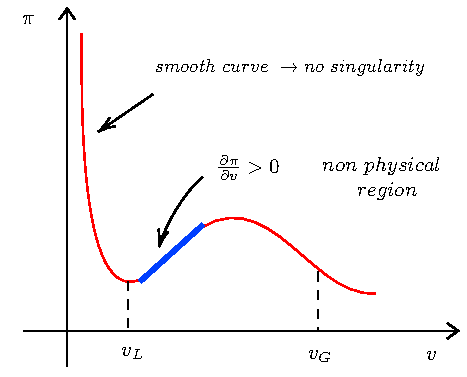
\includegraphics[width=0.7\textwidth]{../lessons/14_image/4.pdf}
\caption{\label{fig:14_3} Van der Waals isotherm for \(T<T_c\).}
\end{figure}


\subsubsection{Equal area or Maxwell construction}
As we have previously anticipated, Maxwell's equal area rule is a method to "manually" remove the unphysical regions of Van der Waals isotherms.

From phase coexistence and general properties of phase transitions we know that at the coexistence of two phases the chemical potentials and the pressures of the two phases must be equal;  furthermore, from thermodynamic potentials we also know that the chemical potential is the Gibbs free energy per particle, namely \(G=\mu N \), and in general we have also:
\begin{equation*}
    \dd[]{G} = - S \dd[]{T} + V \dd[]{P} + \mu \dd[]{N}
\end{equation*}
Now, differentiating \(G=\mu N\) and subtracting this last equation we get:
\begin{equation*}
  \dd[]{\mu } = - \frac{S}{N} \dd[]{T} + \frac{V}{N} \dd[]{P}
\end{equation*}
Therefore, since along an isotherm  \( \dd[]{T}=0\), we will have:
\begin{equation*}
  \dd[]{\mu } = \frac{V}{N} \dd[]{P}
\end{equation*}
At the coexistence we have also \( \dd[]{P}_{coex}= 0  \), hence
\begin{equation*}
  \dd[]{\mu } = 0
\end{equation*}
is the physical condition.
Recall that for Van der Wall \( \dd[]{P} \neq 0  \)!
Hence, the physical coexistence condition implies
\begin{equation*}
  0 = \int_{1}^{2} \dd[]{\mu } = \mu (2) - \mu (1) \overset{Van\, der\, Walls}{=} \frac{1}{N} \int_{P_G}^{P_L} \dd[]{P} V
\end{equation*}
Looking also at the Figure \ref{fig:14_4}, we see that this means that the horizontal segment of the isotherm must be drawn so that the two regions have the same area (from which the name of the method).
The integral can be partitioned in two parts
\begin{equation*}
  0 = \int_{P_G}^{P_L} V \dd[]{P} \quad \Rightarrow \int_{P_G}^{P_x} V\dd[]{P} = - \int_{P_x}^{P_L} \dd[]{P} V
\end{equation*}
Hence, the equal area condition gives the value of \( P_x \) of the coexistence line!

\clearpage

\begin{figure}[h!]
\centering
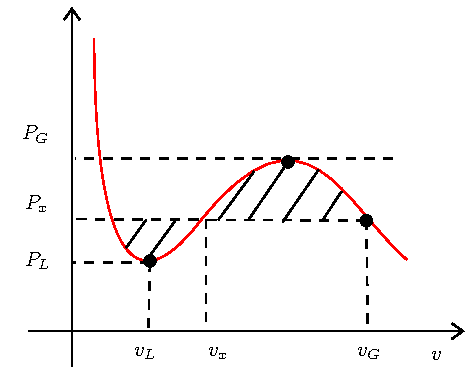
\includegraphics[width=0.6\textwidth]{../lessons/14_image/5.pdf}
\caption{\label{fig:14_4} Maxwell's equal area rule: Van der Walls isotherm for \( T < T_c \).}
\end{figure}




\subsection{Critical exponents of Van der Walls equation}
Let us now study the behaviour of systems obeying Van der Waals equations near the critical point, computing one of the critical exponents.

\subsubsection{\( \pmb{\beta}  \) exponent}
Let us recall that the equation of state is
\begin{equation*}
  \qty(\pi + \frac{3}{\nu ^2}) \qty(3 \nu - 1) = 8 \tau
\end{equation*}
where
\begin{equation*}
  \pi = \frac{P}{P_c}, \quad \nu = \frac{v }{v_c}, \quad \tau = \frac{T}{T_c}
\end{equation*}
Let us consider
\begin{equation}
  \begin{cases}
   t \equiv \tau -1 = \frac{T-T_c}{T_c} \\
   \Phi = \nu -1 = \frac{v-v_c}{v_c}
  \end{cases}
\end{equation}
indeed we want to analyze the deviation from the critical point.
Close to the critical point we have \( \tau \sim \nu \sim 1 \) and \( t \sim \Phi \sim 0 \).

We now expand the equation of state with respect to \( t \) and \( \Phi  \) in the neighbourhood of the critical point:
\begin{equation*}
  \qty(\pi + \frac{3}{(1+\Phi )^2}) \qty(3 (\Phi +1) -1) = 8 (t+1)
\end{equation*}
By rearranging,
\begin{equation*}
  \Rightarrow \pi = \frac{8(t+1)}{2(\Phi +1)-1} - \frac{3}{(1+\Phi )^2}
\end{equation*}
Expanding for \( \Phi \sim 0 \), since we have
\begin{equation*}
  (1+\Phi )^ \alpha \simeq 1 + \alpha \Phi + \frac{\alpha (\alpha -1)}{2!}\Phi ^2 + \frac{\alpha (\alpha -1)(\alpha -2)}{3!}\Phi ^3
\end{equation*}
we obtain
\begin{equation*}
\begin{split}
\pi  &\simeq (1+t)\left(4-6 \Phi  +9\Phi ^{2}-{\frac {27}{2}}\Phi ^{3}+\cdots \right)-(3-6\Phi +9\Phi ^{2}-12\Phi ^{3}+\cdots ) \\
&\sim 1+4t-6\Phi t+9\Phi ^{2}t-{\frac {3}{2}}\Phi ^{3}-{\frac {27}{2}}\Phi ^{3}t+\cdots
\end{split}
\end{equation*}
Finally, the result is
\begin{equation}
  \pi \simeq 1 + 4 t - 6 t \Phi - \frac{3}{2} \Phi ^3 + O (t \Phi ^2,\Phi ^4)
  \label{eq:14_7}
\end{equation}
where the terms we have neglected are justified a posteriori  (i.e. we will see that
\( \Phi \sim t^{1/2} \); we could have not neglected them, but the result of the computation doesn't change).

The strategy we want to apply is the following: since we want to determine how \( \Phi  \)  changes with \( t \), we can determine the relation between the densities \( \Phi_g \) and \( \Phi _l \) in the gaseous and liquid phase from Maxwell's equal area rule. This way, from the expression of \( \pi \) we can determine the pressures in the two phases and express them in terms of \( \Phi_g \)  or \( \Phi _l \), and since \( \pi_l = \pi _g \) at the coexistence we can obtain from this equation the behaviour of \( \Phi  \)  in terms of \( t \).

Hence, as said, in order to get the values of \( v_G (P) \) and \( v_L (P) \) at coexistence, we use the Maxwell construction
\begin{equation*}
  \int_{P_G}^{P_L} v\dd[]{P} = 0
\end{equation*}
and since \( v =  (\Phi +1)v_c \) and \(   \dd[]{P} = P_c \dd[]{\pi }  \) we have:
\begin{equation}
  \int_{liq}^{gas} (\Phi +1) v_c P_c \dd[]{\pi } = 0
    \label{eq:14_5}
\end{equation}
Let us consider \( T < T_c \) fixed (it is true if and only if \( t<0 \), but small), hence
\begin{equation*}
  \pi = \pi (v) = \pi (\Phi )
\end{equation*}
From Eq.\eqref{eq:14_7} we have
\begin{equation*}
  \dd[]{\pi} \simeq - 6 t \dd[]{\Phi } - \frac{9}{2} \Phi ^2 \dd[]{\Phi }
\end{equation*}
Thus the result of the differential \(   \dd[]{P} = P_c \dd[]{\pi }  \) is
\begin{equation*}
   \dd[]{P} = P_c \qty[-6t \dd[]{\Phi } - \frac{9}{2} \Phi ^2 \dd[]{\Phi }  ]
\end{equation*}
Then, from equation \eqref{eq:14_5} we have the integral
\begin{equation}
  \int_{\Phi _l}^{\Phi _g} \Phi \qty(-6t - \frac{9}{2} \Phi ^2) \dd[]{\Phi }  = 0
\end{equation}
hence,
\begin{equation*}
   - 3 \Phi _g^2 \qty[t + \frac{\Phi_g ^2}{g}] + 3 \Phi _l^2 \qty[t + \frac{\Phi _l^2}{g}] = 0
\end{equation*}
Since \( t \) is small we can neglect it, and so:
\begin{equation*}
  \Phi _g^2 = \Phi _l^2 \quad \Rightarrow   \Phi _g = \pm \Phi _l
\end{equation*}
Remembering that:
\begin{equation*}
  \Phi _g = \frac{v_g - v_c}{v_c}, \quad \Phi _l = \frac{v_l - v_c}{v_c}
\end{equation*}
we see that the only acceptable solution is
\begin{equation}
  \Phi _g = - \Phi _l
\end{equation}
(since the volume of a gas is larger than that of a liquid). Therefore, substituting
\( \Phi _g \) and \( \rho _l = - \rho _g \)  into the expression of \( \pi  \) (Eq. \eqref{eq:14_7}), we get
\begin{subequations}
\begin{align*}
  \Phi _g \rightarrow \pi_g  &= 1 + 4 t - 6 t \Phi _g - \frac{3}{2} \Phi _g^3  \\
    \Phi _l \rightarrow \pi_l  &= 1 + 4 t + 6 t \Phi _g + \frac{3}{2} \Phi _g^3
\end{align*}
\end{subequations}
The two expression of \( \pi  \)  must be equal \( \pi _g = \pi _l \) since we are at the coexistence. Solving with respect to \( \Phi _g \) we get
\begin{equation*}
3\rho _g (4t+ \rho _g^2) = 0
\end{equation*}
and excluding of course the case  \( \rho _g = 0 \), in the end:
\begin{equation}
  \Phi _g = 2 \sqrt{-t} \sim \qty(\frac{T_c-T}{T_c})^{1/2}
\end{equation}
which implies
\begin{equation}
  \beta = \frac{1}{2}
\end{equation}



\section{Theories of weakly interacting fluids}
If the gas is not ideal but made by weakly interacting particles, it is possible to follow a \emph{perturbative approach}  to compute the partition function of such systems. Let us consider \( N \) particles in region \( \Omega  \) of volume \( V \). Particles interact through a generic two-body potential that depends only on the relative distance between the particles:
\begin{equation*}
  U_2 ( \va{r}_i, \va{r}_j) = \Phi (\abs{\va{r}_i - \va{r}_j} )
\end{equation*}
Hence,
\begin{equation}
  \Rightarrow U ( \{ \va{r} \}  ) = \frac{1}{2} \sum_{i,j}^{} \Phi (\abs{\va{r}_i - \va{r}_j} )
\end{equation}
Its Hamiltonian will be:
\begin{equation}
  \mathcal{H}_ \Omega (\{ \va{r} \}  ) = \sum_{i=1}^{N} \frac{\va{p}_i^2}{2m} + \sum_{i,j>i}^{} \Phi (\abs{\va{r}_i - \va{r}_j} )
\end{equation}
and its partition function in the canonical ensamble:
\begin{equation}
  Z_ \Omega (N,V,T) = \frac{1}{N! \Lambda ^{3N}} Q_N (V,T)
\end{equation}
where
\begin{equation}
  Q_N (V,T) = \int_{V}^{} \dd[]{\va{r}_1} \int_{V}^{} \dd[]{\va{r}_2} \dots \int_{V}^{} \dd[]{\va{r}_N} \exp [- \beta U (\{ \va{r} \}  )]
\end{equation}
\begin{remark}
Of course for ideal gases \( U = 0 \), and so
\begin{equation*}
  Q_N (V,T) = V^N \quad \rightarrow Z_N^{ideal} = \frac{V^N}{N! \Lambda ^{3N}}
\end{equation*}
and the dependence on \( T \) is exclusively due to \( \Lambda = \Lambda (T) \) (i.e. kinetic energy).
\end{remark}
Now, suppose \( U \neq 0 \), but small!
If we consider also the interaction terms we must insert a correction \( \chi  \) in the configurational contribution to the partition function.
 We can say that our \( Q_N (V,T) \) it would be the on of the ideal version times a new function
\begin{equation}
 Q_N (V,T) \simeq V^N \chi (N,V,T)
\end{equation}
which (depending on the possible presence of attractive terms in the interaction potential \( \Phi  \) can in general be also a function of the temperature \( T \);
furthermore the correction depends strongly on the gas density: if it is low the particles will not "perceive" the presence of the other ones and the ideal gas approximation is a good one, while for high densities the particles will be closer to each other and corrections to \( Q_N \) are necessary.
\begin{remark}
If \( \Phi  \) is only repulsive, \( \chi  \) does not depend on \( T \).
\end{remark}
Let us note that inserting the correction \( \chi  \), the free energy of the system will be:
\begin{equation}
  F_N = F_N^{ideal} - k_B T \ln{\chi }
\end{equation}
As previously said, the correction \( \chi  \) due to particle-particle interaction depends on the particle density \( \rho  \) of the fluid:
\begin{equation}
  \begin{cases}
   \rho _{small} &\Rightarrow  U = 0 \\
   \rho _{high} &\Rightarrow  U \neq 0 \text{ and not negligible}
  \end{cases}
\end{equation}
This suggests that the equation of state of a weakly interacting gas can be expanded formally in powers of \( \rho  \). This is known as \emph{virial expansion}.

In particular, for the ideal gas:
\begin{equation*}
  \frac{P}{k_B T} = \rho
\end{equation*}
For a non ideal gas, let us add the other terms of the expansion
\begin{equation}
  \rightarrow \frac{P}{k_B T} = \rho + B_2 (T) \rho ^2 + B_3 (T)\rho ^3+ \dots + O(\rho ^n)
  \label{eq:14_6}
\end{equation}
this is a virial expansion and it is one of the most used. The coefficient \( B \) are called the \emph{virial coefficients}.
The Eq.\eqref{eq:14_6} was first introduced as a formula to fit experimental data. Indeed, making a fit, you will obtain the virial coefficients. This is what physicist have done for years.  Then, mapping the coefficient with the real world experiments, we can find some macroscopical parameters.
The formula \eqref{eq:14_6} can be also obtained rigorously from a perturbation approach to the partition function (as we will see later). Now, the question is: which is the virial expansion of a Van der Walls (i.e. mean field) gas?


\subsection{Van der Walls and virial expansion}
Let us see for example the virial expansion of the Van der Waals equation. From Van der Waals equation we have:
\begin{equation*}
  \frac{P}{k_B T} = \frac{N}{V-bN} - \frac{a N^2}{k_B T V^2}
\end{equation*}
Let us factorize the term \( (N/V) \),
\begin{equation*}
  \frac{P}{k_B T} = \qty(\frac{N}{V}) \qty(1 - b \frac{N}{V})^{-1} - \frac{a}{k_B T}\qty(\frac{N}{V})^2
\end{equation*}
Then, by expanding in power of \( (N/V) \) and defining \( \rho = N/V \), we have
\begin{equation*}
\begin{split}
  \Rightarrow \frac{P}{k_B T}  &= \qty(\frac{N}{V}) + \qty(\frac{N}{V})^2 \qty(b - \frac{a}{k_B T}) + \qty(\frac{N}{V})^3 b^2 + \qty(\frac{N}{V})^4 b^3 + \dots \\
  & = \rho + \qty(b - \frac{a}{k_B T})\rho ^2 + b^2 \rho ^3 + b^3 \rho ^4 + \dots
\end{split}
\end{equation*}
We can thus immediately identify the first virial coefficient:
\begin{equation*}
  B_2 (T)^{VdW} = b - \frac{a}{k_B T}, \qquad B_3^{VdW} = b^2
\end{equation*}
where in \( B_2 (T)^{VdW}  \) the first term is repulsive on excluded volume and the second one is the attraction term. We note also that \( B_3^{VdW} \) is always positive.

\subsubsection{Boyle's temperature \( T_B \) }
The Boyle's temperature is the \( T \) at which the second coefficient is zero:
\begin{equation*}
  B_2^{VdW} (T_B) = 0
\end{equation*}
so we have removed the most important coefficient. The competiting effects of repulsion and attraction are cancelled out. In this case, the Van der Walls temperature \( T_B^{VdW} \) is
\begin{equation*}
  T_B^{VdW} = \frac{a}{b k_B}
\end{equation*}
to be compared with the critical temperature \( T_c^{VdW} \) that is
\begin{equation*}
  T_c^{VdW} = \frac{8 a}{27 b^3}
\end{equation*}
We notice that \( T_c^{VdW} \ll T_B ^{VdW} \).  It is clear that the Boyle's temperature must be much greater than the critical one.

\begin{remark}
   Consider a polymer, the transition point called the \( \theta  \) point is when the second coefficient is zero, as the case described above, but it is interesting in polymer kind of system (lesson).
\end{remark}

\subsection{Cluster expansion technique for weakly interacting gases}

We now obtain the formal virial expansion by starting from the microscopic system and performing a perturbation expansion of the Boltzmann weights for small values of \( U \).
Let us start from the partition function
\begin{equation}
  Q_N = \int_{V}^{} \dd[]{\va{r}_1} \dots \int_{V}^{} \dd[]{\va{r}_N}  e^{-\beta U (\{ \va{r} \}  ) } = \int_{V}^{} \dd[]{\va{r}_1} \dots \int_{V}^{} \dd[]{\va{r}_N}  e^{-\beta \sum_{i,j > i}^{} \Phi _{ij} }
\end{equation}
where we have used the short notation
\begin{equation*}
  \Phi _{ij} \equiv \Phi (\abs{\va{r}_i - \va{r}_j} )
\end{equation*}
The idea is to find a "small quantity" in terms of which we can expand \( Q_N \); this quantity is the so called \emph{Mayer function}.
\begin{definition}{Mayer function}{}
  The \emph{Mayer f-function} is an auxiliary function that often appears in the series expansion of thermodynamic quantities related to classical many-particle systems. It is defined as
  \begin{equation}
    f (\abs{\va{r}} ) \equiv e^ { - \beta \Phi ( \abs{\va{r}} )} -1
  \end{equation}
  \begin{remark}
  Note: if \( \beta \Phi (r) \ll 1 \), we have \( f(r) \ll 1 \).
  \end{remark}
\end{definition}
In fact, when the gas is ideal  \( f(\va{r}) = 0 \), and if the particles interact weakly \( \Phi  \) is small, and so is \( f(\va{r})  \).
In particular, this expansion will work well for low densities (namely \( | \va {r}_i - \va{r}_j| \)  is large and so \( \Phi  (|\va {r}_i - \va{r}_j| ) \to 0 \)) or high temperatures (namely \( \beta \to 0  \)): in both cases, in fact, \( e^{-\beta  \Phi  (|\va {r}_i - \va{r}_j| )} \rightarrow 1 \) and \( f  (|\va {r}_i - \va{r}_j| ) \to 0 \).
 Using the short notations \(   \Phi _{ij} \equiv \Phi (\abs{\va{r}_i - \va{r}_j} ) \) and \( f_{ij} \equiv f (\abs{\va{r}_i - \va{r}_j} ) \) we have
\begin{equation*}
\begin{split}
  \Rightarrow e^{-\beta \sum_{i}^{}  \sum_{j>i}^{} \Phi _{ij}  } &= \prod_{i}^{} \qty(\prod_{j>i}^{} (1+ f_{ij})  ) \\
  & = \underbrace{(1+f_{12})(1+f_{13})  \dots ( 1 + f_{1N })}_{i=1}   \dots \underbrace{(1+f_{23}) (1+ f_{24}) \dots ( 1 + f_{2N })}_{i=2} \dots \\
  & = (1 + f_{12} + f_{13} + f_{12}f_{13}) (1+f_{14}) \dots(1+f_{23}) \\
  & = 1 + \sum_{i}^{} \sum_{j>i}^{} f_{ij} + \cancel{\sum_{i=1}^{N} \sum_{k \ge i}^{} \sum_{l > k}^{} \sum_{j > i }^{} \sum_{(ij) \neq (lk)}^{}  f_{ij} f_{kl}       } + O (f^3)
\end{split}
\end{equation*}
where
\begin{equation*}
  f_{ij} \equiv  e^{-\beta \Phi _{ij}} -1
\end{equation*}
Higher order terms contain products of \( 3,4,\dots f_{ij} \) terms. For simplicity, let us consider first only linear terms. Hence, the solution is given by considering only the linear term. This is the cluster expansion.





\end{document}
